
        \documentclass[12p]{article}
        \usepackage[margin=1in, left=1.5in, includefoot]{geometry}
        \usepackage{longtable, tabu}
        \usepackage[table, dvipsnames]{xcolor}
        \usepackage{array,booktabs}
        \usepackage{color}
        \usepackage{indentfirst}
        \usepackage{graphicx}
        \usepackage{float}
        \usepackage[utf8]{inputenc}
        \usepackage{listings}
        \usepackage{url}
        \usepackage{multirow}
        \usepackage{seqsplit}
        
        \definecolor{ferrarired}{rgb}{1.0, 0.11, 0.0}
        \definecolor{orange(colorwheel)}{rgb}{1.0, 0.5, 0.0}
        \definecolor{deepskyblue}{rgb}{0.0, 0.75, 1.0}
        \definecolor{grannysmithapple}{rgb}{0.66, 0.89, 0.63}
        \definecolor{gray(x11gray)}{rgb}{0.75, 0.75, 0.75}
        \definecolor{amber}{rgb}{1.0, 0.75, 0.0}
        
        \newcommand{\icon}[1]{\includegraphics[height=12pt]{#1}}
        \newcommand{\hash}[1]{{\ttfamily\seqsplit{#1}}}

        \setlength{\arrayrulewidth}{0.3mm}
\setlength{\tabcolsep}{18pt}
\renewcommand{\arraystretch}{1.5}
\setlength{\parindent}{1em}
\begin{document}
\begin{titlepage}
\begin{center}
\line(1,0){320}\\
[0.25in]
\huge{\bfseries Android Analysis Report}
\line(1,0){320}\\
[0.5in]
\begin{figure}[H]
	\centering
	
\includegraphics[scale=0.5]{/home/miki/Documents/GITHUB/AndroidPermissions/python/vulns/report_icons/logo.png}
\end{figure}
\textsl{\LARGE Demo app}\\
\textsf{\LARGE com.termux}\\
[2.5in]
\end{center}
\begin{flushright}
\textbf{\large Date 2018-06-23}
\end{flushright}
\end{titlepage}
\tableofcontents
\thispagestyle{empty}
\cleardoublepage
\setcounter{page}{1}
\section{Signature}
	\begin{longtable}{p{1.5cm} p{12.5cm} }
\textbf{Owner} & \hash{CN=mobilepearls.com, OU=Unknown, O=Mobile Pearls, L=Unknown, ST=Unknown, C=SE}\\ 
\textbf{Issuer} & \hash{CN=mobilepearls.com, OU=Unknown, O=Mobile Pearls, L=Unknown, ST=Unknown, C=SE}\\ 
\textbf{Serial Number} & \hash{4bc5e4fd}\\ 
\textbf{MD5} & \hash{26:27:7C:2D:20:44:9D:35:4F:7D:70:1A:6E:06:1C:77}\\ 
\textbf{SHA1} & \hash{A9:66:C9:F8:87:F0:E7:EA:85:91:21:68:6F:75:2F:31:D0:69:74:0D}\\ 
\textbf{SHA256} & \hash{73:8F:0A:30:A0:4D:3C:8A:1B:E3:04:AF:18:D0:77:9B:CF:3E:A8:8F:B6:08:08:F6:57:A3:52:18:61:C2:EB:F9}\\ 
\textbf{Algorithm} & \hash{SHA1withRSA}\\ 
	\end{longtable}
\section{PERMISSIONS}
	\begin{longtable}{p{3cm} p{10cm} }
	\rowcolor{grannysmithapple!70} Type & List \\
\hline
Dangerous &  WRITE\_EXTERNAL\_STORAGE \\ 
\hline
Overprivileged &  WAKE\_LOCK \\ 
 &  VIBRATE \\ 
 &  INTERNET \\ 
\hline
\hline
Automatically granted dangerous permissions &  READ\_EXTERNAL\_STORAGE \\ 
\hline
	\end{longtable}
\cleardoublepage
\newpage
\section{FINDINGS SUMMARY}\label{sec:summary}
\begin{figure}[H]
\centering
	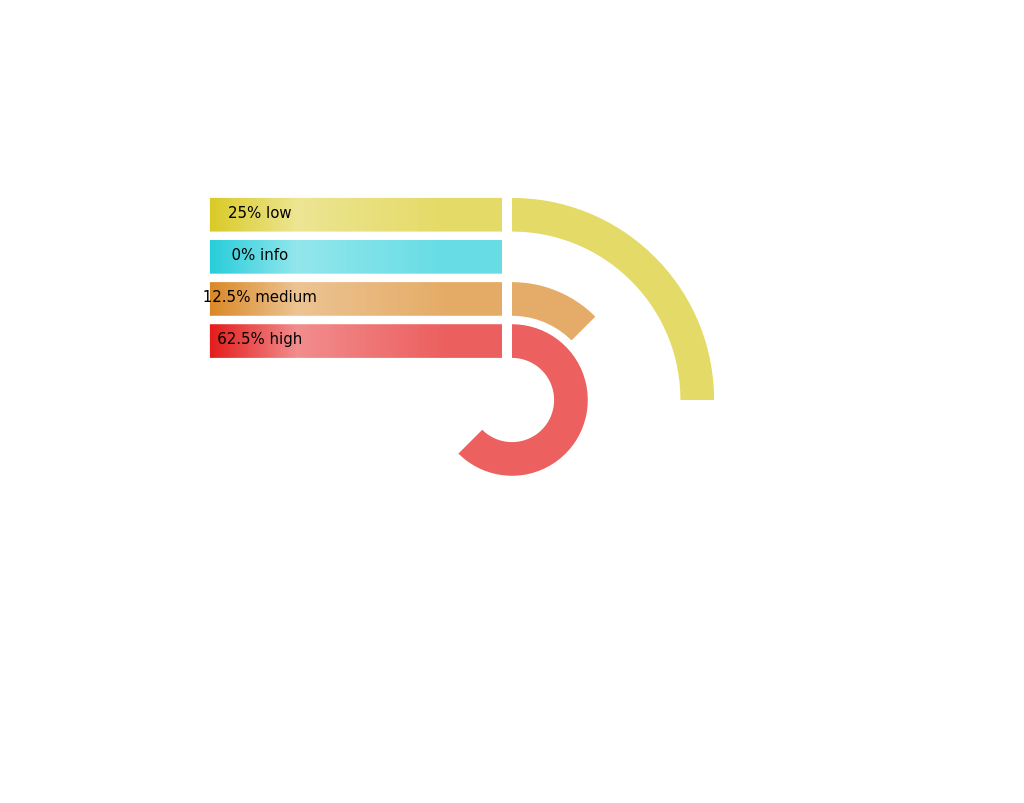
\includegraphics[scale=0.5]{/home/miki/Documents/GITHUB/AndroidPermissions/apks/playstore_apps/com_termux/report/pie_chart.png}
\end{figure}
	\begin{longtable}{p{0.5cm} p{10cm} p{1.5cm}}
	\rowcolor{grannysmithapple!70} Index & Title & Impact \\
	A1&Application is using Logs& \color{amber}\textbf{Low} \\
\hline\\	A2&Application Data can be Backed up& \color{orange(colorwheel)}\textbf{Medium} \\
\hline\\	A3&Launch Mode of Activity \newline (com. termux. app. TermuxActivity) is not standard.& \color{ferrarired}\textbf{High} \\
\hline\\	A4&Activity \newline (com. termux. app. TermuxActivity) is not Protected. An intent-filter exists.& \color{ferrarired}\textbf{High} \\
\hline\\	A5&Activity \newline (com. termux. HomeActivity) is not Protected. An intent-filter exists.& \color{ferrarired}\textbf{High} \\
\hline\\	A6&TaskAffinity is set for Activity \newline (com. termux. filepicker. TermuxFileReceiverActivity)& \color{ferrarired}\textbf{High} \\
\hline\\	A7&Activity \newline (com. termux. filepicker. TermuxFileReceiverActivity) is not Protected. An intent-filter exists.& \color{ferrarired}\textbf{High} \\
\hline\\	A8&Content Provider \newline (com. termux. filepicker. TermuxDocumentsProvider) is protected by a custom permission.& \color{orange(colorwheel)}\textbf{Medium} \\
\hline\\	A9&Content Provider \newline (com. termux. app. TermuxOpenReceiver\$ ContentProvider) is not Protected. [android:exported=true]& \color{ferrarired}\textbf{High} \\
\hline\\	A10&& \color{amber}\textbf{Low} \\
\hline\\	\end{longtable}
\cleardoublepage
\newpage
\section{DETAILED FINDINGS}
\subsection{A1: Application is using Logs}
\subsubsection*{\protect\icon{/home/miki/Documents/GITHUB/AndroidPermissions/python/vulns/report_icons/basic_sheet.png} Description}
Logs were found during the analysis process. When improperly used, they may expose sensitive information such as passwords, usernames, etc.
\subsubsection*{\protect\icon{/home/miki/Documents/GITHUB/AndroidPermissions/python/vulns/report_icons/basic_magnifier.png} Evidence}
\path{/home/miki/Documents/GITHUB/AndroidPermissions/apks/playstore_apps/com_termux/app/smali/android/support/v4/b/a/a.smali
Landroid/util/Log -> i(Ljava/lang/String;Ljava/lang/String;Ljava/lang/Throwable;)}

\path{/home/miki/Documents/GITHUB/AndroidPermissions/apks/playstore_apps/com_termux/app/smali/android/support/v4/b/a/a.smali
Landroid/util/Log -> i(Ljava/lang/String;Ljava/lang/String;Ljava/lang/Throwable;)}

\path{/home/miki/Documents/GITHUB/AndroidPermissions/apks/playstore_apps/com_termux/app/smali/android/support/v4/widget/a.smali
Landroid/util/Log -> e(Ljava/lang/String;Ljava/lang/String;)}

\path{/home/miki/Documents/GITHUB/AndroidPermissions/apks/playstore_apps/com_termux/app/smali/android/support/v4/view/ViewPager.smali
Landroid/util/Log -> e(Ljava/lang/String;Ljava/lang/String;)}

\path{/home/miki/Documents/GITHUB/AndroidPermissions/apks/playstore_apps/com_termux/app/smali/android/support/v4/view/ViewPager.smali
Landroid/util/Log -> w(Ljava/lang/String;Ljava/lang/String;)}

\path{/home/miki/Documents/GITHUB/AndroidPermissions/apks/playstore_apps/com_termux/app/smali/com/termux/terminal/i.smali
Landroid/util/Log -> wtf(Ljava/lang/String;Ljava/lang/String;Ljava/lang/Throwable;)}

\path{/home/miki/Documents/GITHUB/AndroidPermissions/apks/playstore_apps/com_termux/app/smali/com/termux/terminal/i.smali
Landroid/util/Log -> w(Ljava/lang/String;Ljava/lang/String;)}

\path{/home/miki/Documents/GITHUB/AndroidPermissions/apks/playstore_apps/com_termux/app/smali/com/termux/terminal/f.smali
Landroid/util/Log -> e(Ljava/lang/String;Ljava/lang/String;)}

\path{/home/miki/Documents/GITHUB/AndroidPermissions/apks/playstore_apps/com_termux/app/smali/com/termux/terminal/f.smali
Landroid/util/Log -> w(Ljava/lang/String;Ljava/lang/String;)}

\path{/home/miki/Documents/GITHUB/AndroidPermissions/apks/playstore_apps/com_termux/app/smali/com/termux/terminal/f.smali
Landroid/util/Log -> e(Ljava/lang/String;Ljava/lang/String;)}


\textit{snip}
\newline \textsl{For the full list view \path{/home/miki/Documents/GITHUB/AndroidPermissions/apks/playstore_apps/com_termux/report}}
\subsubsection*{\protect\icon{/home/miki/Documents/GITHUB/AndroidPermissions/python/vulns/report_icons/basic_todo.png} Recommendation}

\subsection{A2: Application Data can be Backed up}
\subsubsection*{\protect\icon{/home/miki/Documents/GITHUB/AndroidPermissions/python/vulns/report_icons/basic_sheet.png} Description}
This flag allows anyone to backup your application data via adb. It allows users who have enabled USB debugging to copy application data off of the device.
\subsubsection*{\protect\icon{/home/miki/Documents/GITHUB/AndroidPermissions/python/vulns/report_icons/basic_todo.png} Recommendation}
android:allowBackup = False
\subsection{A3: Launch Mode of Activity (com. termux. app. TermuxActivity) is not standard.}
\subsubsection*{\protect\icon{/home/miki/Documents/GITHUB/AndroidPermissions/python/vulns/report_icons/basic_sheet.png} Description}
An Activity should not be having the launch mode attribute set to "singleTask/singleInstance" as it becomes root Activity and it is possible for other applications to read the contents of the calling Intent.
\subsubsection*{\protect\icon{/home/miki/Documents/GITHUB/AndroidPermissions/python/vulns/report_icons/basic_todo.png} Recommendation}
It is required to use the "standard" launch mode attribute when sensitive information is included in an Intent.
\subsection{A4: Activity (com. termux. app. TermuxActivity) is not Protected. An intent-filter exists.}
\subsubsection*{\protect\icon{/home/miki/Documents/GITHUB/AndroidPermissions/python/vulns/report_icons/basic_sheet.png} Description}
A  Activity is found to be shared with other apps on the device therefore leaving it accessible to any other application on the device. The presence of intent-filter indicates that the Activity is explicitly exported.
\subsubsection*{\protect\icon{/home/miki/Documents/GITHUB/AndroidPermissions/python/vulns/report_icons/basic_todo.png} Recommendation}
It is recommended to set the protection level to signature, so only applications signed with the same certificate can obtain the permission.
\subsection{A5: Activity (com. termux. HomeActivity) is not Protected. An intent-filter exists.}
\subsubsection*{\protect\icon{/home/miki/Documents/GITHUB/AndroidPermissions/python/vulns/report_icons/basic_sheet.png} Description}
A  Activity is found to be shared with other apps on the device therefore leaving it accessible to any other application on the device. The presence of intent-filter indicates that the Activity is explicitly exported.
\subsubsection*{\protect\icon{/home/miki/Documents/GITHUB/AndroidPermissions/python/vulns/report_icons/basic_todo.png} Recommendation}
It is recommended to set the protection level to signature, so only applications signed with the same certificate can obtain the permission.
\subsection{A6: TaskAffinity is set for Activity (com. termux. filepicker. TermuxFileReceiverActivity)}
\subsubsection*{\protect\icon{/home/miki/Documents/GITHUB/AndroidPermissions/python/vulns/report_icons/basic_sheet.png} Description}
If taskAffinity is set, then other application could read the Intents sent to Activities belonging to another task.
\subsubsection*{\protect\icon{/home/miki/Documents/GITHUB/AndroidPermissions/python/vulns/report_icons/basic_todo.png} Recommendation}
Always use the default setting keeping the affinity as the package name in order to prevent sensitive information inside sent or received Intents  from being read by another application.
\subsection{A7: Activity (com. termux. filepicker. TermuxFileReceiverActivity) is not Protected. An intent-filter exists.}
\subsubsection*{\protect\icon{/home/miki/Documents/GITHUB/AndroidPermissions/python/vulns/report_icons/basic_sheet.png} Description}
A  Activity is found to be shared with other apps on the device therefore leaving it accessible to any other application on the device. The presence of intent-filter indicates that the Activity is explicitly exported.
\subsubsection*{\protect\icon{/home/miki/Documents/GITHUB/AndroidPermissions/python/vulns/report_icons/basic_todo.png} Recommendation}
It is recommended to set the protection level to signature, so only applications signed with the same certificate can obtain the permission.
\subsection{A8: Content Provider (com. termux. filepicker. TermuxDocumentsProvider) is protected by a custom permission.}
\subsubsection*{\protect\icon{/home/miki/Documents/GITHUB/AndroidPermissions/python/vulns/report_icons/basic_sheet.png} Description}
A Content Provider is found to be protected by a custom defined permission. The permission can be obtained by malicious apps installed prior to this one. More info at \url{https://github.com/commonsguy/cwac-security/blob/master/PERMS.md}
\subsubsection*{\protect\icon{/home/miki/Documents/GITHUB/AndroidPermissions/python/vulns/report_icons/basic_todo.png} Recommendation}
Failing to protect components could leave them vulnerable to attack by malicious apps.The component should be reviewed for vulnerabilities, such as injection and information leakage. 
\subsection{A9: Content Provider (com. termux. app. TermuxOpenReceiver\$ ContentProvider) is not Protected. [android:exported=true]}
\subsubsection*{\protect\icon{/home/miki/Documents/GITHUB/AndroidPermissions/python/vulns/report_icons/basic_sheet.png} Description}
A Content Provider is found to be shared with other apps on the device therefore leaving it accessible to any other application on the device.
\subsubsection*{\protect\icon{/home/miki/Documents/GITHUB/AndroidPermissions/python/vulns/report_icons/basic_todo.png} Recommendation}
It is recommended to set the protection level to signature, so only applications signed with the same certificate can obtain the permission.
\subsection{A10: }
\subsubsection*{\protect\icon{/home/miki/Documents/GITHUB/AndroidPermissions/python/vulns/report_icons/basic_sheet.png} Description}

\subsubsection*{\protect\icon{/home/miki/Documents/GITHUB/AndroidPermissions/python/vulns/report_icons/basic_magnifier.png} Evidence}
\path{/home/miki/Documents/GITHUB/AndroidPermissions/apks/playstore_apps/com_termux/app/smali/android/support/v4/b/a/a.smali invoke}

\subsubsection*{\protect\icon{/home/miki/Documents/GITHUB/AndroidPermissions/python/vulns/report_icons/basic_todo.png} Recommendation}

\cleardoublepage
\newpage
\section{VISUALIZATIONS}
\subsection{Chord Diagram - Class Relations}
\begin{figure}[H]
	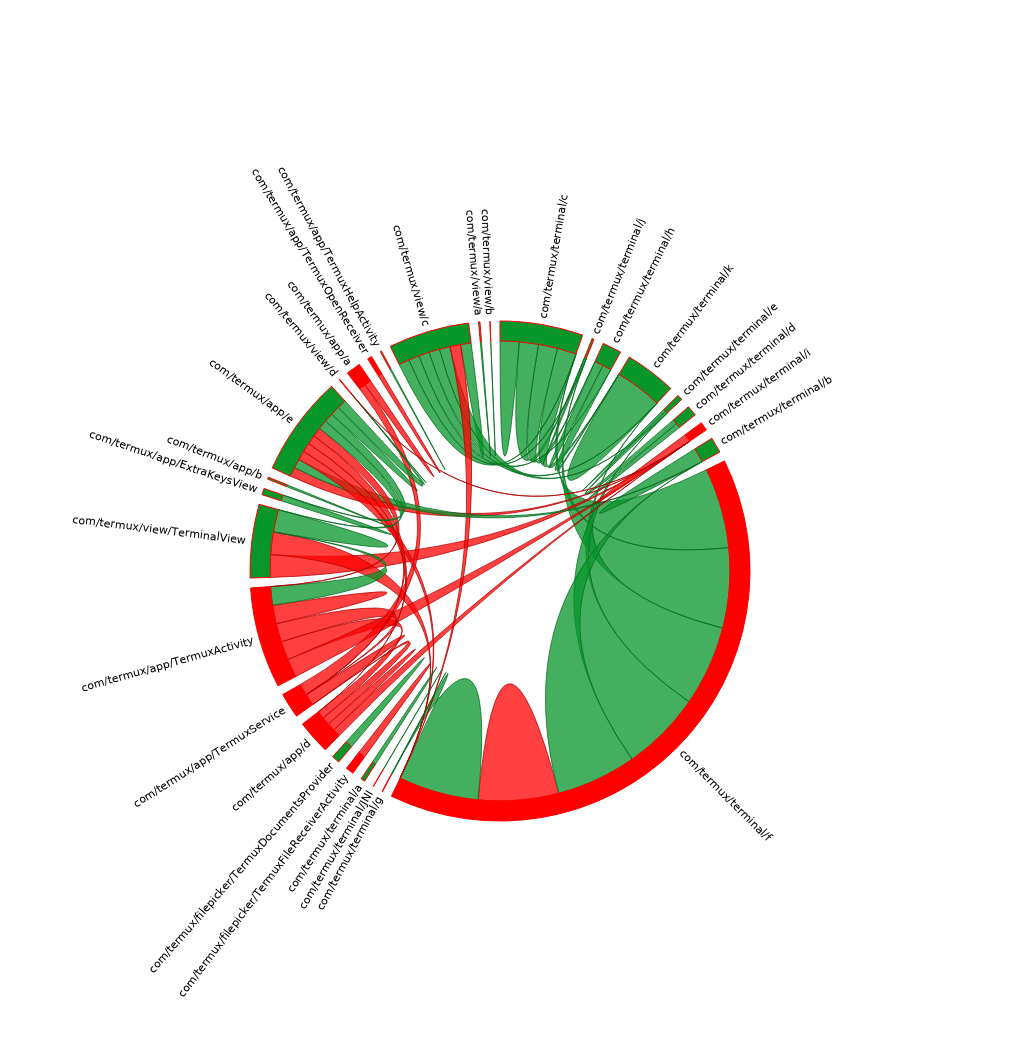
\includegraphics[scale=0.45]{/home/miki/Documents/GITHUB/AndroidPermissions/apks/playstore_apps/com_termux/report/chord_diagram.png}\end{figure}\subsection{Hot Spot - System Overview}
\begin{figure}[H]
\centering
	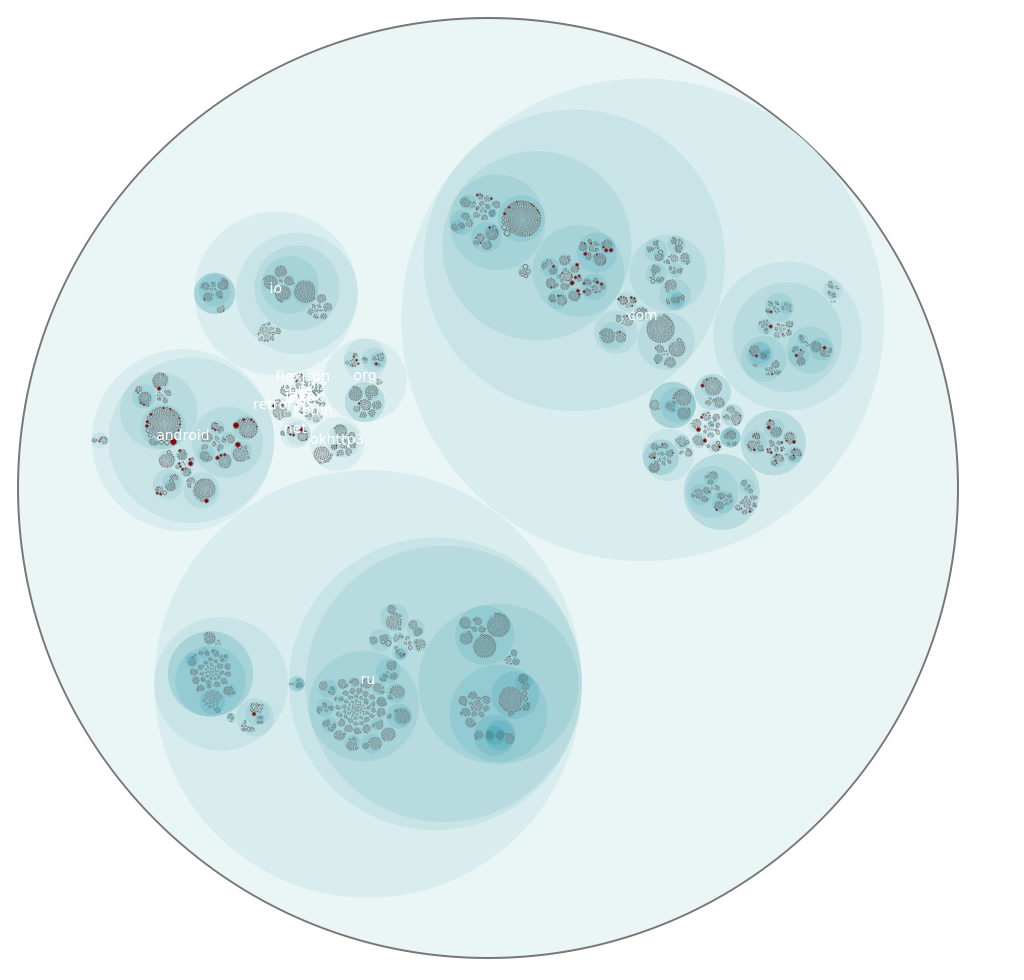
\includegraphics[scale=0.5]{/home/miki/Documents/GITHUB/AndroidPermissions/apks/playstore_apps/com_termux/report/hotspot.png}\end{figure}\begin{longtable}{p{0.3cm} p{12cm}}
\rowcolor{orange} Index & Class \\
1 & \path{/home/miki/Documents/GITHUB/AndroidPermissions/apks/playstore_apps/com_termux/app/smali/android/a/a/c.smali} \\
2 & \path{/home/miki/Documents/GITHUB/AndroidPermissions/apks/playstore_apps/com_termux/app/smali/android/a/a/e.smali} \\
3 & \path{/home/miki/Documents/GITHUB/AndroidPermissions/apks/playstore_apps/com_termux/app/smali/android/a/a/b.smali} \\
4 & \path{/home/miki/Documents/GITHUB/AndroidPermissions/apks/playstore_apps/com_termux/app/smali/android/a/a/d.smali} \\
5 & \path{/home/miki/Documents/GITHUB/AndroidPermissions/apks/playstore_apps/com_termux/app/smali/android/a/a/a.smali} \\
6 & \path{/home/miki/Documents/GITHUB/AndroidPermissions/apks/playstore_apps/com_termux/app/smali/android/a/a/f.smali} \\
7 & \path{/home/miki/Documents/GITHUB/AndroidPermissions/apks/playstore_apps/com_termux/app/smali/android/support/v4/b/a/a.smali} \\
8 & \path{/home/miki/Documents/GITHUB/AndroidPermissions/apks/playstore_apps/com_termux/app/smali/android/support/v4/a/a.smali} \\
9 & \path{/home/miki/Documents/GITHUB/AndroidPermissions/apks/playstore_apps/com_termux/app/smali/android/support/v4/widget/DrawerLayout$e$1.smali} \\
10 & \path{/home/miki/Documents/GITHUB/AndroidPermissions/apks/playstore_apps/com_termux/app/smali/android/support/v4/widget/a$1.smali} \\
	\end{longtable}
\end{document}
